\documentclass[12pt]{article}
\usepackage{amsmath}
\usepackage[margin = 1in]{geometry}
\usepackage{graphicx}
\usepackage{booktabs}
\usepackage{natbib}
\usepackage{lipsum}
\usepackage{setspace}
\usepackage[colorlinks=true, citecolor=blue]{hyperref}
\doublespacing
\title{Machine Learning for Handwriting Recognition: Algorithms and Techniques}
\author{Lai Jiang\\
  University of Connecticut Department of Statistics
}

\begin{document}
\maketitle

\paragraph{Abstract}
Will be Implemented after the article is finished.

\paragraph{Keywords}
Machine Learning, Deep Learning, Handwriting Recognition, Activation Function, Model, Parameters...

\paragraph{Introduction}
In an era where digital communication pervades nearly every facet of our lives, the beauty and uniqueness of human handwriting still holds profound significance. From historical manuscripts to personal notes, handwriting offers a glimpse into a person's individuality and emotions. Yet, deciphering diverse handwritten styles and converting them into digital text is a challenging task. The irregularities, variations, and idiosyncrasies present in handwriting have made its recognition one of the most intriguing problems in the realm of pattern recognition and artificial intelligence. However, the evolution of machine learning, with its robust algorithms and sophisticated techniques, has brought groundbreaking advancements to this domain. Handwriting recognition, once a distant dream, is now manifesting in various applications ranging from mail sorting to bank cheque processing and beyond. This essay delves into the heart of machine learning algorithms and techniques that power handwriting recognition, shedding light on the innovations that bridge the gap between the analog strokes of a pen and the digital bytes of a computer.

\paragraph{Data Collection}
In tackling handwriting recognition tasks, selecting the right libraries and packages is paramount for achieving robust training results. Noteworthy libraries include TensorFlow and Keras which offer a plethora of deep learning functionalities crucial for building and training neural networks adept at recognizing handwritten characters. Additionally, PyTorch is a highly flexible and dynamic open-source machine learning framework that is particularly known for its ease of use and suitability for a variety of tasks, including handwriting recognition. It allows for the construction, training, and evaluation of deep neural networks with a straightforward and Pythonic interface.On the other hand, the MNIST dataset is a classic in the machine learning community, comprising 60,000 training images and 10,000 testing images of handwritten digits from 0 to 9. Each image is grayscale and 28x28 pixels in size. This dataset has been widely used as a benchmark to evaluate and compare different algorithms' performance in the domain of handwriting recognition. When utilized in conjunction with PyTorch, the MNIST dataset can serve as a powerful tool to develop and evaluate handwriting recognition models efficiently. 

\paragraph{Paragraph 3}
In tackling handwriting recognition tasks, selecting the right libraries and packages is paramount for achieving robust training results. Noteworthy libraries include TensorFlow and Keras which offer a plethora of deep learning functionalities crucial for building and training neural networks adept at recognizing handwritten characters. Additionally, PyTorch is a highly flexible and dynamic open-source machine learning framework that is particularly known for its ease of use and suitability for a variety of tasks, including handwriting recognition. It allows for the construction, training, and evaluation of deep neural networks with a straightforward and Pythonic interface.On the other hand, the MNIST dataset is a classic in the machine learning community, comprising 60,000 training images and 10,000 testing images of handwritten digits from 0 to 9. Each image is grayscale and 28x28 pixels in size. This dataset has been widely used as a benchmark to evaluate and compare different algorithms' performance in the domain of handwriting recognition. When utilized in conjunction with PyTorch, the MNIST dataset can serve as a powerful tool to develop and evaluate \begin{figure}
    \centering
    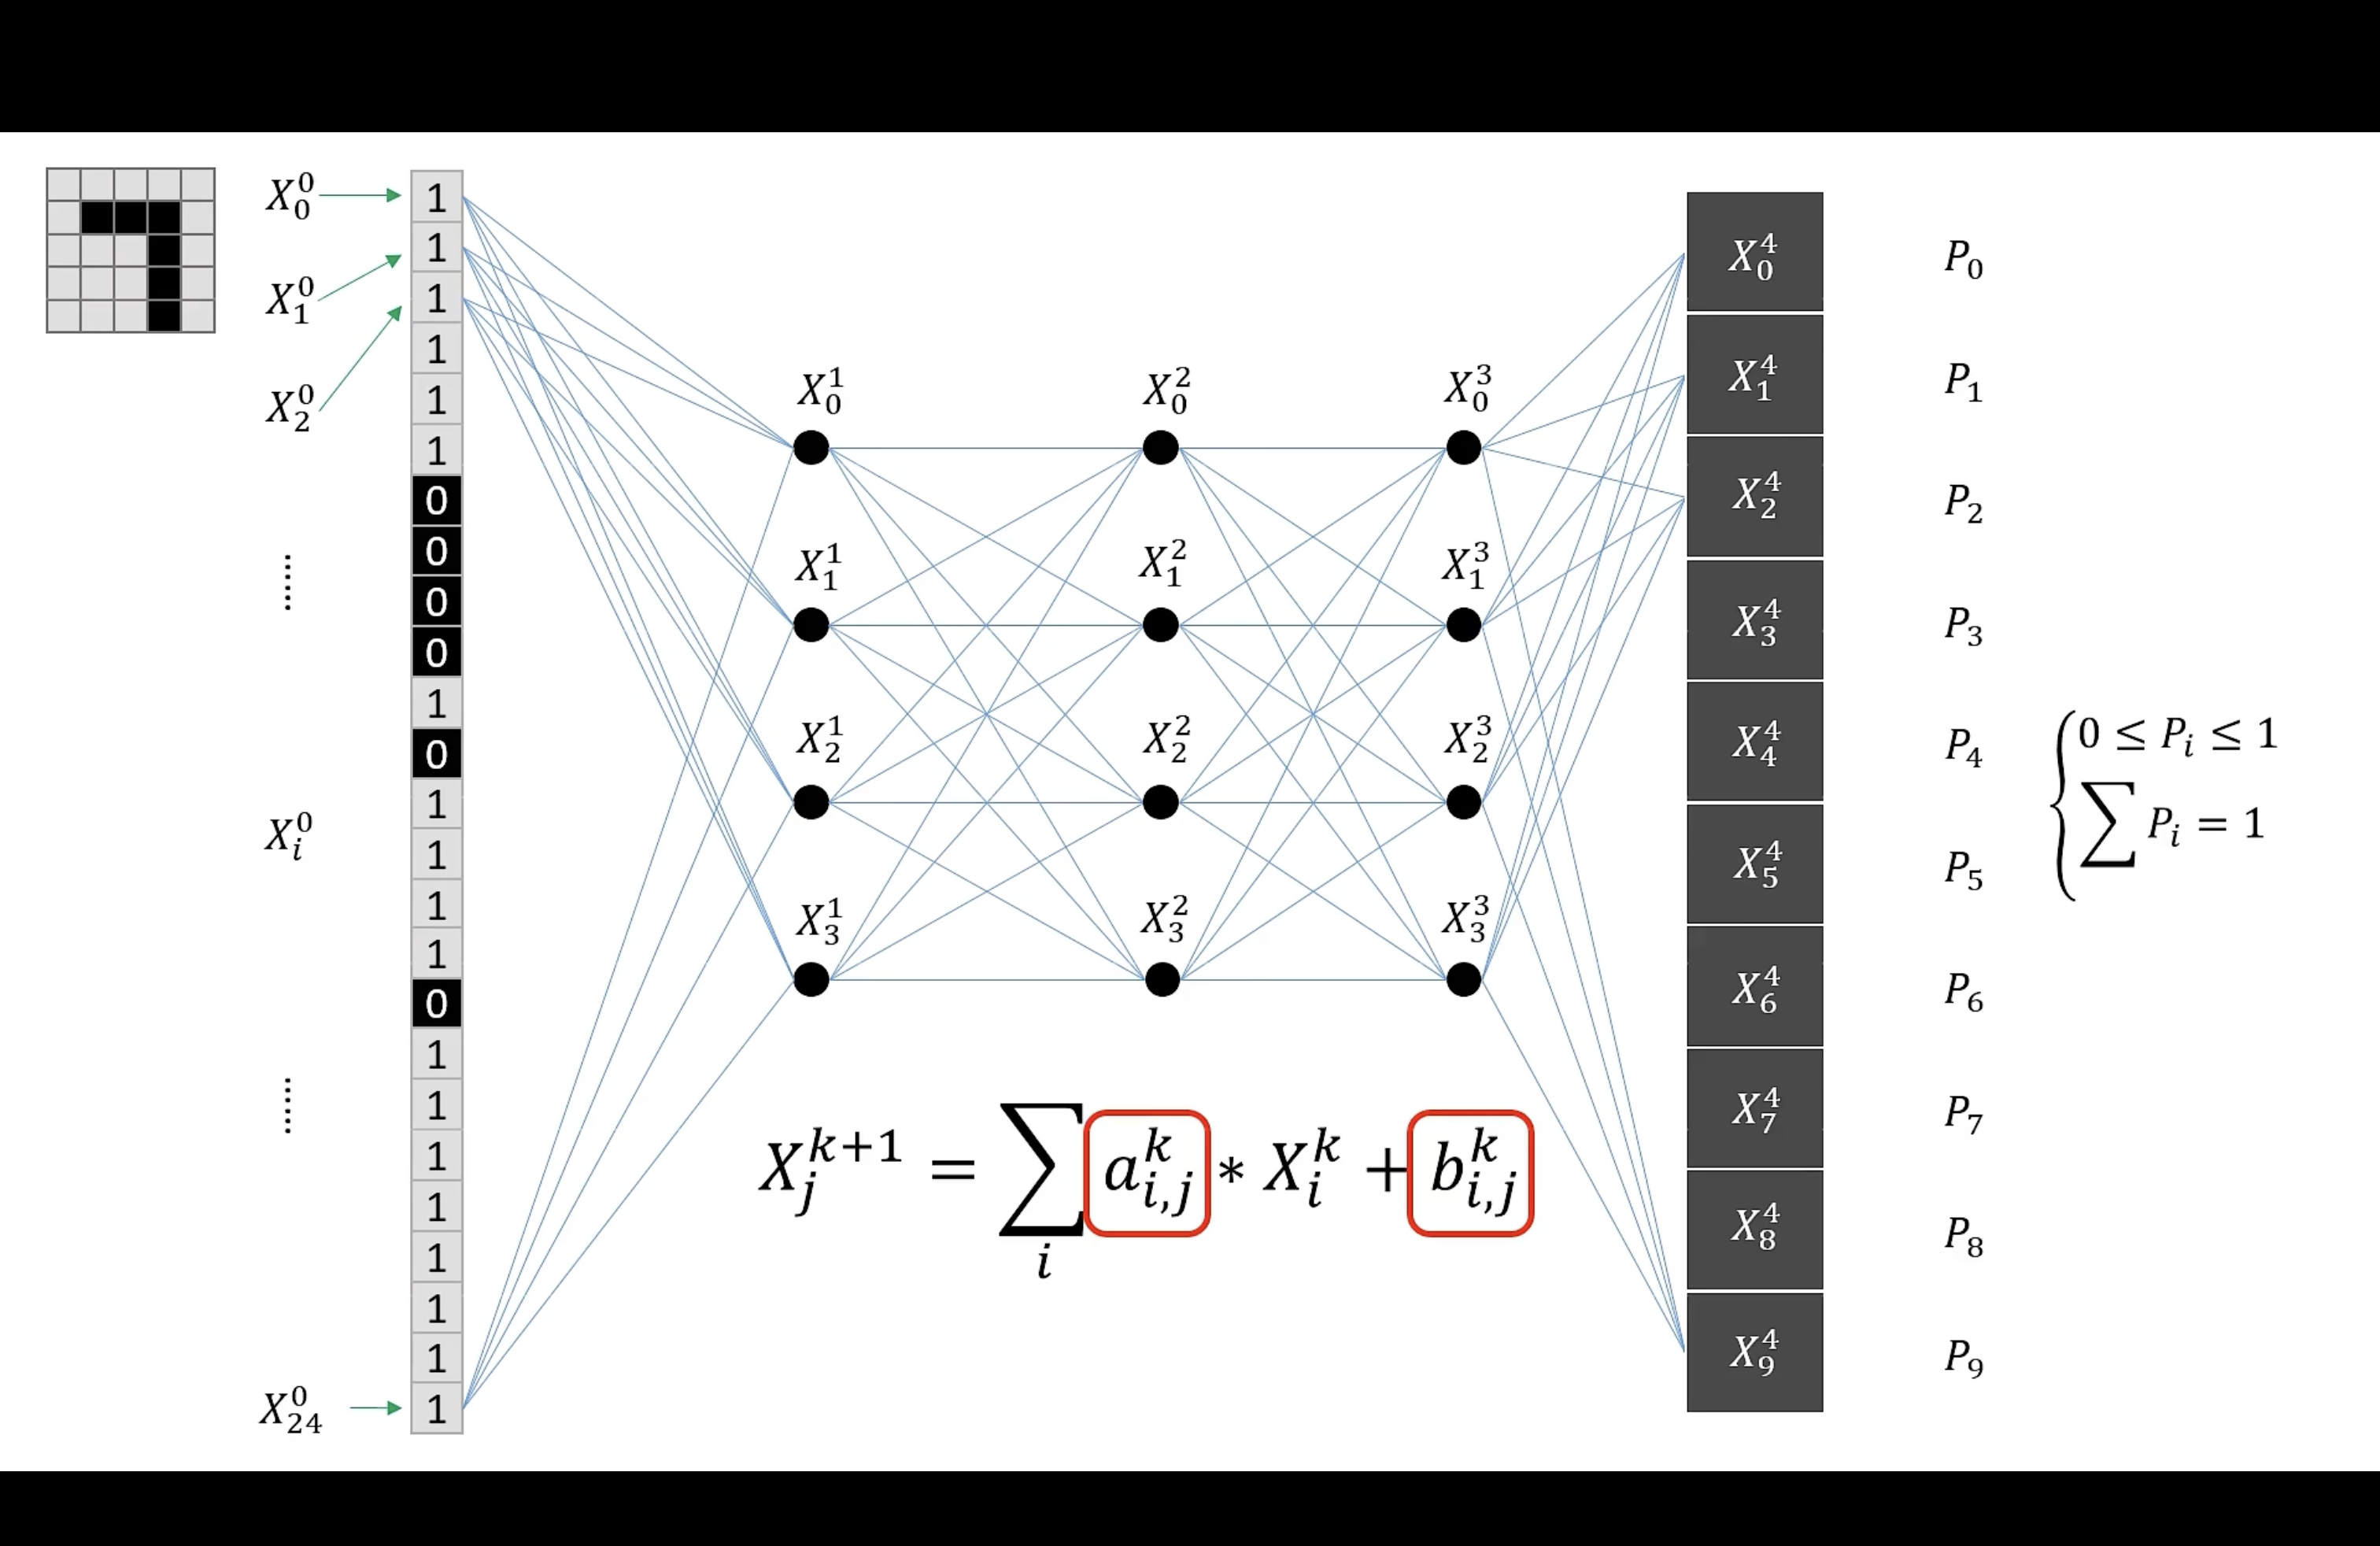
\includegraphics[width=0.5\textwidth]{Image1.png}
    \vspace{0.5cm}
    \caption{This is an example of Nerual Network}
    \label{fig:my_image_label}
\end{figure}


\paragraph{Paragraph 4}


\bibliographystyle{plain}
\bibliography{Citations.bib}
\cite{824821}
\cite{NIPS2008_66368270}
\cite{6981034}
\end{document}